\chapter{IMPLEMENTASI}
	Bab ini membahas mengenai implementasi dari sistem yang sudah di desain dan dirancang pada bab sebelumnya. Pembahasan secara rinci akan dijelaskan pada setiap komponen yang ada yaitu \textit{load generator}, pengambil data uji beban dan \textit{service controller} yang meliputi \textit{web service}, basis data dan \textit{task queue}.
	
	\section{Lingkungan Implementasi}
		Dalam mengimplementasikan sistem pada tugas akhir ini, digunakan beberapa perangkat pendukung sebagai berikut.
		
		\subsection{Perangkat Keras}
		Perangkat keras yang digunakan dalam pengembangan sistem adalah sebagai berikut:
		\begin{enumerate}
			\item \textit{Web service} dan \textit{task queue}, \textit{processor} AMD FX-7600P Radeon R7, 12 Compute Cores 4C+8G dan RAM 8GB.
			\item \textit{Node swarm} dengan IP 167.71.194.235, \textit{processor} Intel(R) Xeon(R) CPU E5-2650 v4@2.20GHz dan RAM 4GB.
			\item \textit{Node swarm} dengan IP 165.22.55.82, \textit{processor} Intel(R) Xeon(R) CPU E5-2650 v4@2.20GHz dan RAM 4GB.
			\item \textit{Node swarm} dengan IP 167.71.194.233, \textit{processor} Intel(R) Xeon(R) CPU E5-2650 v4@2.20GHz dan RAM 4GB.
			\item Basis data \textit{MySQL} dengan IP 178.128.123.143, \textit{processor} Intel(R) Xeon(R) Gold 6140 CPU@2.30GHz dan RAM 1GB.
		\end{enumerate}
	
		\subsection{Perangkat Lunak}
		Perangkat lunak yang digunakan dalam pengembangan sistem adalah sebagai berikut:
		\begin{enumerate}
			\item Sistem Operasi \textit{Ubuntu} 18.04 LTS 64 Bit
			\item \textit{Docker} versi 18.09.6 
			\item \textit{Headless Chrome} 
			\item \textit{Puppeteer} versi 0.12.0
			\item \textit{NPM} versi 6.4.1
			\item \textit{Node.js} versi 8.15.1
			\item \textit{Python} versi 3.6.8
			\item \textit{MySQL} Ver 14.14 Distrib 5.7.26
			\item \textit{Shell Script}
			\item \textit{PHP} dan \textit{Laravel} versi 5.8
		\end{enumerate}
		
	\section{Implementasi \textit{Load Generator}}
		Berdasarkan perancangan dan desain, \textit{load generator} merupakan aktor yang akan berfungsi menggantikan pengguna ketika mengakses ke web. \textit{Load generator} yang akan digunakan adalah \textit{Docker}, namun diperlukan beberapa tahap untuk bisa menggunakan \textit{Docker} atau kontainer sebagai \textit{load generator}, yaitu tahap pemasangan dan konfigurasi. Tahap pemasangan \textit{Docker} dapat dilihat di Kode Sumber \ref{instalasidocker}, sedangkan untuk konfigurasi akan dibagi menjadi beberapa tahap yaitu:
		\begin{enumerate}
			\item Pembuatan \textit{Docker Image}
			\item Pembuatan lingkungan kontainer
			\item Pemasangan \textit{Headless Chrome} dan \textit{Puppeteer}
		\end{enumerate}
			
		\subsection{Implementasi Pembuatan \textit{Docker Image}}
			\textit{Docker Image} digunakan untuk menjalankan kontainer, pada tugas akhir ini \textit{Docker Image} akan dibuat terlebih dahulu agar bisa digunakan untuk menjalankan \textit{Puppeteer} dan \textit{Headless Chrome}. Namun untuk membuat \textit{Docker Image} diperlukan beberapa tahapan yaitu konfigurasi \texttt{Dockerfile}, pemasangan \textit{Docker Compose} dapat dilihat pada Kode Sumber \ref{dockercomposeinstall} dan konfigurasi \texttt{docker-compsoe.yml} dan unggah \textit{Docker Image} ke \textit{Docker Hub}.
			
			\indent Konfigurasi \texttt{Dockerfile} dapat dilihat pada Kode Sumber \ref{dockerimage}, sedangkan konfigurasi \texttt{docker-compose.yml} dapat dilihat pada Kode Sumber \ref{dockercompose}.
				\begin{lstlisting}[frame=single,tabsize=2,breaklines,caption={Konfigurasi \textit{Dockerfile} },label=dockerimage, captionpos=b, language=json]
	FROM node:8
	RUN apt-get update
	# for https
	RUN apt-get install -yyq ca-certificates
	# install libraries
	RUN apt-get install -yyq libappindicator1 libasound2 libatk1.0-0 libc6 libcairo2 libcups2 libdbus-1-3 libexpat1 libfontconfig1 libgcc1 libgconf-2-4 libgdk-pixbuf2.0-0 libglib2.0-0 libgtk-3-0 libnspr4 libnss3 libpango-1.0-0 libpangocairo-1.0-0 libstdc++6 libx11-6 libx11-xcb1 libxcb1 libxcomposite1 libxcursor1 libxdamage1 libxext6 libxfixes3 libxi6 libxrandr2 libxrender1 libxss1 libxtst6
	# tools
	RUN apt-get install -yyq gconf-service lsb-release wget xdg-utils
	RUN apt-get install -yyq fonts-liberation 
	COPY code /app/code
	COPY output /app/output
	WORKDIR /app/code
	RUN yarn install
				\end{lstlisting}
				
				\begin{lstlisting}[frame=single,tabsize=2,breaklines,caption={Konfigurasi \textit{docker-compose.yml} },label=dockercompose, captionpos=b, language=json]
	version: '3'
	services:
		puppeteer:
			build: .
			shm_size: '1gb'
			entrypoint: ["sh", "-c", "sleep infinity"]
				\end{lstlisting}
				
				Kemudian jalankan perintah \textit{Docker Compose} berikut untuk pembuatan \textit{Docker Image}.
				\begin{lstlisting}[frame=single,tabsize=2,breaklines,caption={Perintah untuk menjalankan  \textit{Docker Compose}},label=createimg, captionpos=b, language=json,numbers=none]
	$ docker-compose up
				\end{lstlisting}
				
				Setelah \textit{Docker Image} terbuat, ubah nama \textit{Docker Image} tersebut dan melakukan \textit{commit} agar bisa di \textit{push}. Perintah pada kode sumber \ref{pushimagedocker} yang digunakan oleh penulis ketika mengunggah \textit{Docker Image} ke \textit{Docker Hub}.
				\begin{lstlisting}[frame=single,tabsize=2,breaklines,caption={Perintah untuk mengunggah \textit{Docker Image}},label=pushimagedocker, captionpos=b, language=json,numbers=none]
	$ docker tag puppeteer_puppeteer:latest cphikmawan/ta2019:newpupp
	
	$ docker push cphikmawan/ta2019:newpupp
				\end{lstlisting}
				
		\subsection{Implementasi Pembuatan Lingkungan Kontainer}
			Kontainer akan dipasangkan pada suatu lingkungan yang bisa mengatur segala aktivitas kontainer, lingkungan yang akan dibangun pada sistem menggunakan alat orkestrasi yaitu \textit{Docker Swarm}. Untuk mengimplementasikan \textit{Docker Swarm} pada sistem ini, dibutuhkan satu \textit{node host} sebagai \textit{manager node} dan dua lainnya sebagai \textit{worker}. Tahap pertama yang dilakukan yaitu menginisiasi salah satu \textit{node host} yang akan digunakan sebagai \textit{manager node}. Perintah inisiasi \textit{manager node} terdapat pada Kode Sumber \ref{swarminit}.
			\begin{lstlisting}[frame=single,tabsize=2,breaklines,caption={Perintah untuk inisiasi \textit{manager node}},label=swarminit, captionpos=b, language=json,numbers=none]
	$ docker swarm init --advertise-addr [IP NODE]
			\end{lstlisting}
			
			Setelah perintah pada kode sumber \ref{swarminit} dijalankan, maka \textit{manager node} akan menghasilkan sebuah token yang digunakan oleh \textit{node host} yang lain untuk bergabung sebagai \textit{worker}. Perintah yang harus dijalankan pada setiap \textit{node host} yang lain terdapat pada Kode Sumber \ref{swarmjoin}.
			\begin{lstlisting}[frame=single,tabsize=2,breaklines,caption={Perintah untuk bergabung ke \textit{Swarm}},label=swarmjoin, captionpos=b, language=json,numbers=none]
	$ docker swarm join --token [token] [IP MANAGER]:2377
			\end{lstlisting}
			
			Tahap terakhir yang dilakukan yaitu memastikan semua \textit{node host} sudah tergabung dengan \textit{manager node}.
			\begin{lstlisting}[frame=single,tabsize=2,breaklines,caption={Perintah untuk melihat daftar \textit{Swarm Node}},label=dockernodels, captionpos=b, language=json,numbers=none]
	$ docker node ls
			\end{lstlisting}
			
		\subsection{Implementasi Pemasangan \textit{Headless Chrome} dan \textit{Puppeteer}}
			\textit{Headless Chrome} dan \textit{Puppeteer} akan dipasang pada masing-masing kontainer menggunakan \textit{Docker Image} yang telah dibuat sebelumnya, untuk pemasangannya akan dilakukan dilingkungan \textit{Docker Swarm} dan dilakukan pada \textit{manager node}. Namun untuk implementasinya dibutuhkan beberapa persiapan dan konfigurasi yang harus dilakukan terlebih dahulu yaitu konfigurasi unduh \textit{Docker Image}, konfigurasi membuat \textit{Docker Network}, konfigurasi \textit{puppeteer.yml}, konfigurasi \textit{deployment}.
			
			\indent Untuk mengunduh \textit{Docker Image} dilakukan pada setiap \textit{node host} menggunakan perintah pada Kode Sumber \ref{unduhimage} dan membuat \textit{Docker Network} pada Kode Sumber \ref{createnetwork}. Sedangkan konfigurasi \texttt{puppeteer.yml} dapat dilihat di Kode Sumber \ref{puppyaml}
			\begin{lstlisting}[frame=single,tabsize=2,breaklines,caption={Perintah untuk mengunduh \textit{Docker Image} },label=unduhimage, captionpos=b, language=json,numbers=none]
	$ docker image pull cphikmawan/ta2019:puppeteer
			\end{lstlisting}
			
			\begin{lstlisting}[frame=single,tabsize=2,breaklines,caption={Perintah untuk membuat\textit{ Docker Network} },label=createnetwork, captionpos=b, language=json,numbers=none]
	$ docker network create \
		--driver overlay \
		--subnet 10.0.0.0/18 \
		--attachable \
		[nama_network]
			\end{lstlisting}
			
			\begin{lstlisting}[frame=single,tabsize=2,breaklines,caption={Konfigurasi \textit{puppeteer.yml}},label=puppyaml, captionpos=b, language=json]
	version: '3'
	# konfigurasi service
	services:
		# nama service yang akan dibuat
		puppeteer:
			# docker image yang digunakan
			image: cphikmawan/ta2019:newpupp
			# sinkronisasi penyimpanan antara kontainer dengan host
			volumes:
				- ./output:/app/output
				- ./code:/app/code
			# direktori kerja didalam kontainer
			working_dir: /app/code
			# konfigurasi untuk jumlah kontainer dan handling
			deploy:
				replicas: 1000
				restart_policy:
					condition: on-failure
			# entrypoint awal tidak akan melakukan apapun
			entrypoint: ["sh", "-c", "sleep infinity"]
	# konfigurasi jaringan
	networks:
		default:
			# jaringan default akan diubah ke jaringan eksternal
			external:
				# akan terkonek ke jaringan "swarm-network"
				name: swarm-network
			\end{lstlisting}
			
			\indent Tahap selanjutnya adalah konfigurasi \textit{deployment} dengan menjalankan perintah yang ditunjukkan pada Kode Sumber \ref{pemasanganstack} di terminal \textit{manager node}
			\begin{lstlisting}[frame=single,tabsize=2,breaklines,caption={Perintah untuk pemasangan kontainer },label=pemasanganstack, captionpos=b, language=json,numbers=none]
	$ docker stack deploy --compose-file=puppeteer.yml [nama_stack]
			\end{lstlisting}
	
	\section{Implementasi Pengambil Data Uji Beban}
		Pengambil Data Uji Beban akan dilakukan menggunakan sebuah pustaka \textit{Node} yaitu \textit{Puppeteer}. Pada saat dilakukan uji beban, \textit{Puppeteer} akan mengambil data uji beban dari \textit{Headless Chrome} menggunakan \textit{API} dari \textit{Puppeteer} secara otomatis. Beberapa data uji beban yang akan diambil yaitu:
		\begin{enumerate}
			\item \textit{Response End} \\
				Atribut ini menunjukkan waktu setelah \textit{user} menerima \textit{byte} terakhir dari dokumen sebelum koneksi transportasi ditutup.
			\item \textit{DOM Content Loaded} \\
				Atribut ini menunjukkan waktu setelah dokumen sudah diterima oleh \textit{user}.
			\item \textit{Load Event End} \\
				Atribut ini mengembalikan waktu ketika memuat dokumen selesai.
			\item \textit{CSS Tracing End} \\
				Atribut ini menunjukkan waktu dari ekstraksi akhir file \textit{CSS} dimuat.
			\item \textit{First Meaningfulpain} \\
				Atribut ini adalah atribut khusus yang ada pada \textit{Chrome} yang menunjukkan bahwa segala konten halaman yang dimuat sudah ditampilkan di layar. \\
		\end{enumerate}
	 
	 	\indent Selain data uji beban diatas, \textit{Puppeteer} juga digunakan untuk mengambil sebuah tangkapan layar sesuai skenario yang dikirimkan oleh pengguna dan mengambil data saat terjadi kegagalan saat memuat \textit{assets} yang tertulis pada \textit{console browser}. Adapun \textit{pseudocode} untuk melakukan pengambilan data uji beban dapat dilihat pada Kode Sumber \ref{pseudocodepupp}.
	 	
	 	\begin{lstlisting}[frame=single,tabsize=2,breaklines,caption={\textit{Pseudocode Puppeteer}},label=pseudocodepupp, captionpos=b, language=json]
 	Variable Declaration
 	Data = Read Scenario File Configuration
 	
 	TESTPAGE FUNCTION:
 		CALL HELPERS FUNCTION:
 			GET Navigation Start
 		START Trace CSS Data
 		Trying to Accessing Website
 		END Trace CSS Data
 		CALL HELPERS FUNCTION:
 			GET Extracted Performance Data
 			GET Extracted CSS Tracing
 			RETURN Extracted Data
 	END TESTPAGE FUNCTION
 	
 	HELPERS FUNCTION:
 		GET Navigation Start
 			RETURN Navigation Start
 		Extracted Performance Data = Performance Data * 1000 - Navigation Start
 			RETURN Extracted Performance Data
 		Extracted CSS Tracing = CSS Tracing / 1000
 			RETURN Extracted CSS Tracing 
 	End Helpers Function
 	
 	MAIN FUNCTION:
 		START Headless Browser
 		GET Error Console
 			RETURN Data to Database
 		TRY:
 			CALL TESTPAGE FUNCTION(Data):
 				Get Data From TestPage -> Save Data Uji Beban
 			GET Page Screenshoot -> Save Screenshoot
 		CATCH ERROR:
 			GET Error
 			GET Page Screenshoot -> Save Screenshoot
 	END MAIN FUNCTION
	 	\end{lstlisting}
	
	\section{Implementasi \textit{Service Controller}}
		Berdasarkan desain dan perancangan, \textit{service controller} terdiri dari komponen \textit{web service}, basis data dan \textit{task queue}. Komponen tersebut akan diimplementasikan pada satu komputer milik penulis yang akan digunakan untuk \textit{web service} dan penggunaan \textit{task queue}, serta satu buah server untuk basis data \textit{MySQL}.
		
		\subsection{Implementasi \textit{Web Service}}
			Pada implementasi \textit{web service} dibutuhkan beberapa persiapan lingkungan yang perlu dilakukan, urutannya meliputi langkah-langkah berikut:
			\begin{enumerate}
				\item Instalasi \textit{PHP}
				\item Instalasi \textit{Composer}
				\item Instalasi \textit{Laravel} versi 5.8
				\item Instalasi \textit{MySQL}
			\end{enumerate}
			
			\indent \textit{Web service} akan menggunakan bahasa \textit{PHP} dan kerangka kerja \textit{Laravel} versi 5.8, sedangkan \textit{Composer} berfungsi untuk memanajemen instalasi pustaka pada \textit{PHP} dan untuk penyimpanan data yang digunakan pada sistem akan disimpan pada basis data \textit{MySQL}. \textit{Web service} berfungsi untuk memudahkan pengguna melakukan uji beban pada suatu web. Tampilan antarmuka pengguna ditunjukkan pada Gambar \ref{gambarweb}.
			
			\begin{figure}[H]
				\centering
				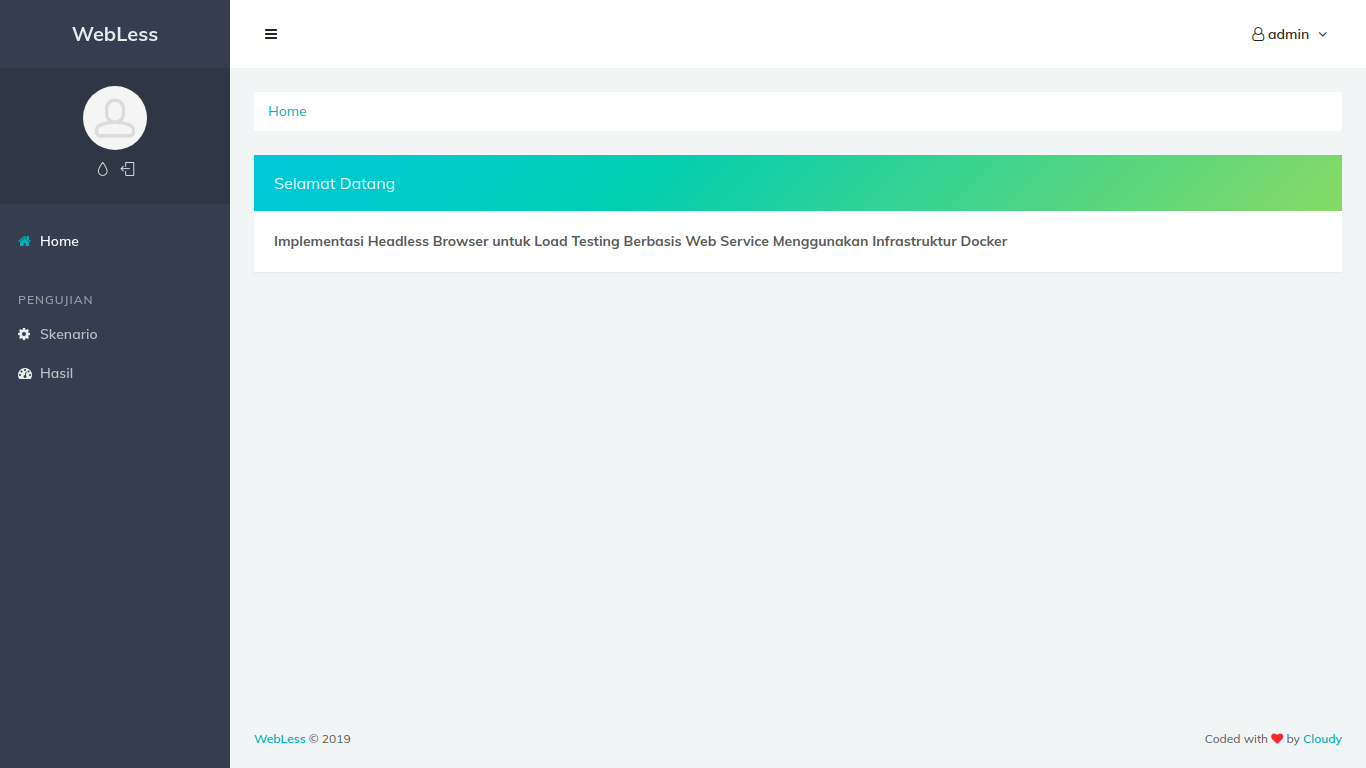
\includegraphics[width=10cm,height=6cm]{Images/C-4/gambarweb.png}
				\caption{Tampilan web antarmuka pengguna}
				\label{gambarweb}
			\end{figure}
			
			\indent \textit{Web service} memiliki beberapa rute \textit{HTTP} yang akan digunakan oleh pengguna ketika mengakses web sistem. Rute-rute tersebut ditunjukkan pada Tabel \ref{tabelruteweb}.
			\begin{longtable}{|p{0.05\textwidth}|p{0.25\textwidth}|p{0.30\textwidth}|p{0.30\textwidth}|}
				\caption{Rute \textit{HTTP} pada \textit{web service}} \label{tabelruteweb} \\ \hline
				\textbf{No} & \textbf{Rute} & \textbf{Metode} & \textbf{Aksi} \\ \hline
				\endhead
				\endfoot
				\endlastfoot
				1 & / & GET & Mengakses halaman \textit{home} \\ \hline
				2 & /login & GET & Mengakses halaman \textit{login} \\ \hline
				3 & /login & POST & Melakukan \textit{login} \\ \hline
				4 & /logout & GET & Melakukan \textit{logout} \\ \hline
				5 & /skenario & GET & Melihat skenario \\ \hline
				6 & /skenario & POST & Menambahkan skenario \\ \hline
				7 & /skenario & DELETE & Menghapus skenario \\ \hline
				8 & /worker & GET & Mengakses halaman \textit{worker} \\ \hline
				9 & /worker & POST & Menambahkan jumlah \textit{worker(load generator)} dan data antrian \\ \hline
				10 & /hasil/rata-rata & GET & Mendapatkan hasil pengujian \\ \hline
				11 & /hasil/error-console & GET & Mendapatkan \textit{error console} web \\ \hline
				12 & /hasil/images & GET & Melihat tangkapan layar web \\ \hline
				13 & /antrian & GET & Melihat jumlah dan status antrian \\ \hline
				
			\end{longtable}
		
		\subsection{Implementasi Skema Basis Data}
			Berdasarkan hasil perancangan basis data pada bab sebelumnya. Data yang dibutuhkan dan digunakan oleh sistem akan disimpan di dalam basis data \textit{MySQL}. Data yang disimpan adalah data \textit{node host swarm}, data kontainer, data pengguna, data skenario pengujian, data antrian \textit{request}, data hasil pengujian, data \textit{error console}, data rata-rata hasil pengujian.
			
			\subsubsection{Tabel \textit{Swarms}}
				Pada tabel \textit{swarms} menyimpan data-data dari node host yang tergabung dilingkungan \textit{swarm}. Berikut definisi tabel \textit{swarms} pada Tabel \ref{tabelswarms}.
				
				\begin{longtable}{|p{0.05\textwidth}|p{0.30\textwidth}|p{0.20\textwidth}|p{0.35\textwidth}|}
					\caption{Tabel \textit{swarms}} \label{tabelswarms} \\
					\hline
					\textbf{No} & \textbf{Kolom} & \textbf{Tipe} & \textbf{Keterangan} \\ \hline
					\endhead
					\endfoot
					\endlastfoot
					1 & id & bigint(20) & Sebagai \textit{primary key}, nilai awal adalah \textit{auto\_increment}. \\ \hline
					2 & swarm\_ip & varchar(255) & Menunjukkan \textit{IP} dari \textit{node host} \\ \hline
					3 & swarm\_username & varchar(255) & Menunjukkan \textit{username} dari \textit{node host} \\ \hline
					4 & swarm\_password & varchar(255) & Menunjukkan \textit{password} dari \textit{node host} \\ \hline
					5 & is\_used & smallint(6) & Menunjukkan status dari \textit{node host} \\ \hline
				\end{longtable}
		
			\subsubsection{Tabel \textit{Containers}}
				Padata tabel \textit{containers} menyimpan data-data dari \textit{Docker Container} yang akan digunakan sebagai \textit{load generator}. Berikut definisi tabel \textit{containers} pada Tabel \ref{tabelcontainers}.
				
				\begin{longtable}{|p{0.05\textwidth}|p{0.30\textwidth}|p{0.20\textwidth}|p{0.35\textwidth}|}
					\caption{Tabel \textit{containers}} \label{tabelcontainers} \\
					\hline
					\textbf{No} & \textbf{Kolom} & \textbf{Tipe} & \textbf{Keterangan} \\ \hline
					\endhead
					\endfoot
					\endlastfoot
					1 & id & bigint(20) & Sebagai \textit{primary key}, nilai awal adalah \textit{auto\_increment} \\ \hline
					2 & task\_id & varchar(100) & Menunjukkan \textit{task id} dari kontainer \\ \hline
					3 & node\_id & varchar(100) & Menunjukkan \textit{node id} tempat kontainer dipasang \\ \hline
					4 & container\_id & varchar(100) & Menunjukkan \textit{id} dari kontainer \\ \hline
					5 & node\_ip & varchar(100) & Menunjukkan \textit{IP} tempat kontainer dipasang \\ \hline
					6 & node\_host & varchar(100) & Menunjukkan \textit{hostname} tempat kontainer dipasang \\ \hline
					7 & status & smallint(6) & Menunjukkan \textit{flag} status dari \textit{container} \\ \hline
					8 & username & varchar(100) & Menunjukkan status kontainer yang sedang digunakan \textit{user} \\ \hline
				\end{longtable}
		
			\subsubsection{Tabel \textit{Users}}
				Pada tabel \textit{users} menyimpan data-data pengguna web yang disediakan sistem. Berikut definisi tabel \textit{users} pada Tabel \ref{tabelusers}. Data pengguna juga memiliki \textit{constraint} dan disimpan pada Tabel \textit{role\_user} \ref{tabelroleuser} dan Tabel \textit{roles} \ref{tabelroles}.
				
				\begin{longtable}{|p{0.05\textwidth}|p{0.30\textwidth}|p{0.20\textwidth}|p{0.35\textwidth}|}
					\caption{Tabel \textit{users}} \label{tabelusers} \\
					\hline
					\textbf{No} & \textbf{Kolom} & \textbf{Tipe} & \textbf{Keterangan} \\ \hline
					\endhead
					\endfoot
					\endlastfoot
					1 & id & bigint(20) & Sebagai \textit{primary key}, nilai awal adalah \textit{auto\_increment} \\ \hline
					2 & name & varchar(255) & Menunjukkan nama pengguna \\ \hline
					3 & email & varchar(255) & Menunjukkan \textit{email} pengguna \\ \hline
					4 & username & varchar(255) & Menunjukkan \textit{username} pengguna \\ \hline
					5 & password & varchar(255) & Menunjukkan \textit{password} pengguna \\ \hline
				\end{longtable}
			
				\begin{longtable}{|p{0.05\textwidth}|p{0.30\textwidth}|p{0.20\textwidth}|p{0.35\textwidth}|}
					\caption{Tabel \textit{role\_user}} \label{tabelroleuser} \\
					\hline
					\textbf{No} & \textbf{Kolom} & \textbf{Tipe} & \textbf{Keterangan} \\ \hline
					\endhead
					\endfoot
					\endlastfoot
					1 & id & bigint(20) & Sebagai \textit{primary key}, nilai awal adalah \textit{auto\_increment} \\ \hline
					2 & role\_id & int(10) & Menunjukkan \textit{id role} pengguna \\ \hline
					3 & user\_id & int(10) & Menunjukkan \textit{id} pengguna \\ \hline
				\end{longtable}
				
				\begin{longtable}{|p{0.05\textwidth}|p{0.30\textwidth}|p{0.20\textwidth}|p{0.35\textwidth}|}
					\caption{Tabel \textit{roles}} \label{tabelroles} \\
					\hline
					\textbf{No} & \textbf{Kolom} & \textbf{Tipe} & \textbf{Keterangan} \\ \hline
					\endhead
					\endfoot
					\endlastfoot
					1 & id & bigint(20) & Sebagai \textit{primary key}, nilai awal adalah \textit{auto\_increment} \\ \hline
					2 & name & varchar(255) & Menunjukkan nama \textit{role} \\ \hline
					3 & description & varchar(255) & Menunjukkan deskripsi hak akses dari nama \textit{role} \\ \hline
				\end{longtable}
		
			\subsubsection{Tabel \textit{Scenarios}}
				Pada tabel \textit{scenarios} menyimpan data-data skenario yang telah dibuat oleh pengguna. Berikut definisi tabel \textit{scenarios} pada Tabel \ref{tabelscenarios}.
			
				\begin{longtable}{|p{0.05\textwidth}|p{0.30\textwidth}|p{0.20\textwidth}|p{0.35\textwidth}|}
					\caption{Tabel scenarios} \label{tabelscenarios} \\
					\hline
					\textbf{No} & \textbf{Kolom} & \textbf{Tipe} & \textbf{Keterangan} \\ \hline
					\endhead
					\endfoot
					\endlastfoot
					1 & id & bigint(20) & Sebagai \textit{primary key}, nilai awal adalah \textit{auto\_increment} \\ \hline
					2 & scenario\_id & varchar(255) & Menunjukkan skenario \textit{id} sebagai \textit{foreign key} \\ \hline
					3 & username & varchar(255) & Menunjukkan keterangan pengguna pembuat skenario \\ \hline
					4 & scenario\_method & varchar(255) & Menunjukkan metode uji \\ \hline
					5 & scenario\_link & varchar(255) & Menunjukkan \textit{link} \textit{website} yang diuji \\ \hline
					6 & scenario\_worker & varchar(255) & Menunjukkan jumlah \textit{load generator} yang diinginkan pengguna \\ \hline
					7 & scenario\_status & smallint(6) & Menunjukkan status skenario, nilai awal adalah 0 \\ \hline
				\end{longtable}
		
			\subsubsection{Tabel \textit{Queues}}
				Pada tabel \textit{queues} menyimpan data-data antrian request yang dilakukan oleh semua pengguna. Berikut definisi tabel \textit{queues} pada Tabel \ref{tabelqueues}.
			
				\begin{longtable}{|p{0.05\textwidth}|p{0.30\textwidth}|p{0.20\textwidth}|p{0.35\textwidth}|}
					\caption{Tabel \textit{queues}} \label{tabelqueues} \\
					\hline
					\textbf{No} & \textbf{Kolom} & \textbf{Tipe} & \textbf{Keterangan} \\ \hline
					\endhead
					\endfoot
					\endlastfoot
					1 & id & bigint(20) & Sebagai \textit{primary key}, nilai awal adalah \textit{auto\_increment} \\ \hline
					2 & created\_at & timestamp & Menunjukkan waktu pembuatan \textit{queue} \textit{request} oleh pengguna \\ \hline
					3 & username & varchar(255) & Menunjukkan keterangan pengguna pembuat \textit{request} \\ \hline
					4 & worker & int(11) & Menunjukkan jumlah \textit{load generator} yang diinginkan pengguna \\ \hline
					5 & status & smallint(6) & Menunjukkan status dari \textit{queue}, nilai awal adalah 0 \\ \hline
				\end{longtable}
		
			\subsubsection{Tabel \textit{Results}}
				Pada tabel \textit{results} menyimpan data-data hasil uji beban yang dilakukan oleh kontainer dan \textit{Puppeteer}. Berikut definisi tabel \textit{results} pada Tabel \ref{tabelresults}.
				
				\begin{longtable}{|p{0.05\textwidth}|p{0.30\textwidth}|p{0.20\textwidth}|p{0.35\textwidth}|}
					\caption{Tabel \textit{results}} \label{tabelresults} \\
					\hline
					\textbf{No} & \textbf{Kolom} & \textbf{Tipe} & \textbf{Keterangan} \\ \hline
					\endhead
					\endfoot
					\endlastfoot
					1 & id & bigint(20) & Sebagai \textit{primary key}, nilai awal adalah \textit{auto\_increment} \\ \hline
					2 & scenario\_id & varchar(255) & Menunjukkan skenario \textit{id} sebagai \textit{foreign key} \\ \hline
					3 & link & varchar(255) & Menunjukkan \textit{link} website yang diuji \\ \hline
					4 & method & varchar(100) & Menunjukkan metode uji \\ \hline
					5 & worker & varchar(255) & Menunjukkan jumlah \textit{load generator} yang diinginkan pengguna \\ \hline
					6 & username & varchar(100) & Menunjukkan keterangan pengguna pembuat \textit{request} \\ \hline
					7 & host & varchar(100) & Menunjukkan \textit{IP node host} yang digunakan kontainer penguji \\ \hline
					8 & response\_end & varchar(100) & Menunjukkan hasil uji response time dalam satuan \textit{ms} \\ \hline
					9 & dom\_content\_load & varchar(100) & Menunjukkan hasil uji waktu memuat \textit{DOM} web dalam satuan \textit{ms} \\ \hline
					10 & load\_event\_end & varchar(100) & Menunjukkan hasil uji \textit{load time} dalam satuan \textit{ms} \\ \hline
					11 & css\_trace\_end & varchar(100) & Menunjukkan hasil uji waktu memuat \textit{css time} dalam satuan \textit{ms} \\ \hline
					12 & first\_meaningful & varchar(100) & Menunjukkan hasil uji waktu memuat konten utama dalam satuan \textit{ms} \\ \hline
					13 & status & smallint(6) & Menunjukkan status apakah untuk proses rata-rata, nilai awal adalah 0 \\ \hline
				\end{longtable}
		
			\subsubsection{Tabel \textit{Errors}}
				Pada tabel \textit{errors} menyimpan data-data kegagalan yang terekam pada \textit{console browser} ketika diakses didalam \textit{Headless Chrome}. Berikut definisi tabel \textit{errors} pada Tabel \ref{tabelerrors}.
				
				\begin{longtable}{|p{0.05\textwidth}|p{0.30\textwidth}|p{0.20\textwidth}|p{0.35\textwidth}|}
					\caption{Tabel \textit{errors}} \label{tabelerrors} \\
					\hline
					\textbf{No} & \textbf{Kolom} & \textbf{Tipe} & \textbf{Keterangan} \\ \hline
					\endhead
					\endfoot
					\endlastfoot
					1 & id & bigint(20) & Sebagai \textit{primary key}, nilai awal adalah \textit{auto\_increment} \\ \hline
					2 & scenario\_id & varchar(255) & Menunjukkan skenario \textit{id} sebagai \textit{foreign key} \\ \hline
					3 & link & varchar(255) & Menunjukkan \textit{link website} yang diuji \\ \hline
					4 & worker & varchar(255) & Menunjukkan jumlah \textit{load generator} yang diinginkan pengguna \\ \hline
					5 & username & varchar(100) & Menunjukkan keterangan pengguna pembuat \textit{request} \\ \hline
					6 & host & varchar(100) & Menunjukkan \textit{IP node host} yang digunakan kontainer penguji \\ \hline
					7 & type & varchar(100) & Menunjukkan tipe \textit{error} \\ \hline
					8 & text & varchar(255) & Menunjukkan keterangan \textit{error} \\ \hline
					9 & args & varchar(255) & Menunjukkan argumen \textit{error} \\ \hline
					10 & location\_url & varchar(255) & Menunjukkan lokasi \textit{url error} \\ \hline
				\end{longtable}
		
			\subsubsection{Tabel \textit{Summary Results}}
				Pada tabel \textit{summary\_results} menyimpan data perhitungan rata-rata dari hasil uji beban yang sudah disimpan pada tabel \textit{results}. Tabel ini yang akan dibuat sebagai laporan uji beban yang disampaikan ke pengguna. Berikut definisi tabel \textit{summary\_results} pada Tabel \ref{tabelsumresults}.
			
				\begin{longtable}{|p{0.05\textwidth}|p{0.30\textwidth}|p{0.20\textwidth}|p{0.35\textwidth}|}
					\caption{Tabel \textit{summary\_results}} \label{tabelsumresults} \\
					\hline
					\textbf{No} & \textbf{Kolom} & \textbf{Tipe} & \textbf{Keterangan} \\ \hline
					\endhead
					\endfoot
					\endlastfoot
					1 & id & bigint(20) & Sebagai \textit{primary key}, nilai awal adalah \textit{auto\_increment} \\ \hline
					2 & scenario\_id & varchar(255) & Menunjukkan \textit{skenario id} sebagai \textit{foreign key} \\ \hline
					3 & link & varchar(255) & Menunjukkan \textit{link website} yang diuji \\ \hline
					4 & method & varchar(100) & Menunjukkan metode uji \\ \hline
					5 & worker & varchar(255) & Menunjukkan jumlah \textit{load generator} yang diinginkan pengguna \\ \hline
					6 & username & varchar(100) & Menunjukkan keterangan pengguna pembuat \textit{request} \\ \hline
					7 & error & varchar(100) & Menunjukkan presentase kegagalan saat dilakukan uji beban \\ \hline
					8 & response\_end & varchar(100) & Menunjukkan rata-rata hasil uji \textit{response time} dalam satuan \textit{ms} \\ \hline
					9 & dom\_content\_load & varchar(100) & Menunjukkan rata-rata hasil uji waktu memuat \textit{DOM} web dalam satuan \textit{ms} \\ \hline
					10 & load\_event\_end & varchar(100) & Menunjukkan rata-rata hasil uji \textit{load time} dalam satuan \textit{ms} \\ \hline
					11 & css\_trace\_end & varchar(100) & Menunjukkan rata-rata hasil uji waktu memuat \textit{css time} dalam satuan \textit{ms} \\ \hline
					12 & first\_meaningful & varchar(100) & Menunjukkan rata-rata hasil uji waktu memuat konten utama dalam satuan \textit{ms} \\ \hline
				\end{longtable}
			
		\subsection{Implementasi \textit{Task Queue}}
			\textit{Task queue} akan digunakan untuk mengatur antrian \textit{request} dari pengguna, pada tugas akhir ini implementasi \textit{task queue} akan dipasang pada komputer yang sama dengan \textit{web service}. Bahasa pemrograman yang akan digunakan untuk mengimplementasikan \textit{task queue} adalah bahasa pemrograman \textit{Python}, sedangkan untuk basis data akan terkoneksi dengan basis data \textit{MySQL} yang terpasang pada server yang berbeda. Selain itu \textit{task queue} akan dijalankan setiap 1 menit sekali pada \textit{crontab}. Selama \textit{task queue} berjalan algoritmenya akan selalu melakukan pengecekan apakah ada antrian yang bisa dieksekusi. \textit{Pseudocode} untuk \textit{task queue} tertera pada Kode Sumber \ref{pseudotaskqueue} dan untuk konfigurasi \textit{crontab} pada Kode Sumber \ref{crontab}.
			
			\begin{lstlisting}[frame=single,tabsize=2,breaklines,caption={\textit{Pseudocode task queue} },label=pseudotaskqueue, captionpos=b, language=json]
	Connection
	
	Variable Declaration

	DECLARE ADDITIONAL FUNCTION
		Get Data Task Queue from MySQL <- LIMIT 1
		RETURN data
	
	MAIN FUNCTION
		Data = CALL ADDITIONAL FUNCTION
		IF Data Not NULL
			Do Task Queue Job
		Else
		 RETURN Null to Output File
	END FUNCTION
			\end{lstlisting}
			
			\begin{lstlisting}[frame=single,tabsize=2,breaklines,caption={Konfigurasi \textit{crontab} },label=crontab, captionpos=b, language=json]
	* * * * * /usr/bin/python3 queue.py >> output.log 2>&1
			\end{lstlisting}